%%%%%%%%%%%%%%%%%%%%%%%%%%%%%%%%%%%%%%%%%%%%%%%%%%%%%%%%%%%%
%%%%%%%%%%%%%%%%%%%%%%%%%%%%%%%%%%%%%%%%%%%%%%%%%%%%%%%%%%%%
\chapter{Spectral Interpretation as a Statistical Mechanics Problem}
\label{chap:alg}
\nopagebreak
%%%%%%%%%%%%%%%%%%%%%%%%%%%%%%%%%%%%%%%%%%%%%%%%%%%%%%%%%%%%
%%%%%%%%%%%%%%%%%%%%%%%%%%%%%%%%%%%%%%%%%%%%%%%%%%%%%%%%%%%%

We have seen in the previous chapter the strategy underlying protein sequencing
by MS/MS, the interpretation problems that have to be faced, and the present
methods to deal with them.
We have also seen the pros and cons of the two approaches to MS/MS spectra
interpretation: database-search and \emph{de-novo} sequencing, and have discussed the
issue of the statistical significance of the score of the reported precursor
sequence.

Basically, all sequencing algorithms, both database-searching and \emph{de-novo}, yield
as a result the solution with the highest score (or, equivalently, with the
lowest energy, if we define an energy as the negative score): from this point of
view, the only difference between them is given by the state-space of the
search, which is just the database in the former case, or all the sequence space
of a given mass in the latter.
Therefore, we can say that they find the ground-state, or zero-temperature
solution, in the appropriate sequence space. Suboptimal solutions, as proposed
in the ranked list, corresponding to the excited states, are not included in the
solution, but listed a part.
On the other hand, physical intuition suggests that, given a reasonable energy
function to score the match between a proposed sequence and the experimental
spectrum, poor quality spectra, with a low signal/noise value (defined in some
suitable sense), should correspond to high energy and/or high entropy. Indeed, a
high number of excited states at small gap from the ground state, representing
alternative solutions with essentially the same energy as the best one, should
point at a bad prediction, possibly related to missing peaks, to the presence of
many or intense noise peaks, or both.

These observations suggest that the introduction of an artificial temperature in
the solutions space, and the study of the resulting thermodynamic equilibrium,
could provide some valuable internal indication of the quality of the
interpretation, in a sense analogous to the False Predictive Rate mentioned in
Section~\ref{sec:reliability}.
For instance, despite the fact that, in a finite system, the existence of real
phase transition is precluded, we could expect that, for each spectrum, there is a
low-temperature phase, where one or a few sequences dominate as candidate
solutions, while at high temperature a ``paramagnetic'' phase exists,
corresponding to a mixture of a huge amount of solutions. The temperature of
transition between the two regimes, as signalled, for instance, by a peak in the
heat capacity, could bring, again, important information on the robustness of
the interpretation -- the higher the temperature, the more reliable the
identification.

In order to exploit the benefits of moving out from the zero-temperature
solution, we need first of all a proper way to map the problem of spectra
interpretation on that of finding the thermodynamic equilibrium of a suitable
physical system, and second, an effective way to actually perform calculations.
In the following, we will deal with both issues: first we will introduce a
discrete unidimensional system, whose states encode all possible amino-acid
sequences of appropriate length. Second, we will define the general form of the
energy function of the model in term of just on-site and next-neighbors
interaction, involving some constraints on the  class of scoring function that
can be implemented in the model. We will leave the detailed derivation of a
particular form of the energy function, inspired by Bayesian modelling, for
Chapter~\ref{chap:pot}, moving forward to introduce a transfer-matrix technique that
allows to calculate exactly the partition function of the model, finding its
equilibrium solution. We will finally discuss how the equilibrium results can be
mapped back to  MS spectra interpretation.

%%%%%%%%%%%%%%%%%%%%%%%%%%%%%%%%%%%%%%%%%%%%%%%%%%%%%%%%%%%%%%%%%%%%%%%%%%%%%%%
\section{Encoding the sequence space on a 1D lattice model}
\label{sec:variables}

A peak in the experimental spectrum gives information on the $m/z$ ratio of the
N- or C-terminal ions (if we neglect the possibility of internal fragments)
obtained in the fragmentation process during CID: such information is not
related to detailed sequence of the fragment ions (even if it can be affected by
the presence of some amino-acid, as we will detail below), but just depends on
the mass and charge of the whole fragment.

We can use this fact to avoid the book-keeping of a combinatorial number of
possible sequences, and to define a physical system whose site variables carry
information on the mass and charge, as well as some other overall quantities
that we will need to characterize completely the parent peptide.
  
Despite the fact that the fragment masses are incommensurable, their
discretization in terms of a unit mass $\eta$, roughly equal to an atomic mass
unit, is a reasonable and natural approximation. Therefore, we define a discrete
one-dimensional lattice  of $M+1$ sites, numbered from $0$ to $M$, where $M$ is
the discretized mass of the parent peptide (more precisely, it is the sum of the
masses of the residues that compose it, neglecting the extra groups H and OH at
the N- and C- term, and neglecting the extra proton of the precursor MH$^+$).
The lattice spacing $\eta$ is given by:
\begin{equation}
\eta=
\sum_{a}\frac{m_{a}^m}{m_{a}}f(a)
=1.0005022782 \,\,,
\end{equation}
the weighted mean of the ratio between the  mono-isotopic residue mass
$m^m_{a}$ and the discrete mass $m_{a}$, where the weight $f(a)$ is the
natural abundance of the residue $a$.

Table \ref{tab:residues} lists  all the residues with their mono-isotopic mass and the corresponding 
discretized value. Testing the model, in Chapter~\ref{chap:msms-results}, we will ignore
post-translational modification and will deal just with sequences made up of
natural amino-acids; however, the following discussion holds valid when PTMs are
present, by simply augmenting Table~\ref{tab:residues} with the corresponding modified
residues masses and corresponding properties.

\begin{table}
\centering
\begin{tabular}{ccccccccc}
\hline \hline
$a$ & $m^m_{a}$ & $m_{a}$ & $f(a)$ & $q$ & $l_1$ & $l_2$ & $l_3$ & $l_4$\\
\hline	
G &  57.021 &  57 & 7.49 & 0 & 0 & 0 & 0 & 0 \\
A &  71.037 &  71 & 5.22 & 0 & 0 & 0 & 0 & 0 \\
S &  87.032 &  87 & 4.53 & 0 & 1 & 0 & 0 & 0 \\
P &  97.053 &  97 & 5.22 & 0 & 0 & 0 & 0 & 0 \\
V &  99.068 &  99 & 1.82 & 0 & 0 & 0 & 0 & 0 \\
T & 101.048 & 101 & 6.26 & 0 & 1 & 0 & 0 & 0 \\
C & 103.009 & 103 & 4.11 & 0 & 0 & 0 & 0 & 0 \\
I & 113.084 & 113 & 7.10 & 0 & 0 & 0 & 0 & 0 \\
L & 113.084 & 113 & 2.23 & 0 & 0 & 0 & 0 & 0 \\
N & 114.043 & 114 & 5.45 & 0 & 0 & 0 & 0 & 0 \\
D & 115.027 & 115 & 9.06 & 0 & 0 & 0 & 0 & 0 \\
Q & 128.059 & 128 & 5.82 & 0 & 0 & 1 & 0 & 0 \\
E & 129.043 & 129 & 2.27 & 0 & 0 & 0 & 0 & 0 \\
M & 131.040 & 131 & 3.91 & 0 & 0 & 0 & 0 & 0 \\
H & 137.059 & 137 & 5.12 & 1 & 0 & 0 & 1 & 0 \\
F & 147.068 & 147 & 7.34 & 0 & 0 & 0 & 0 & 0 \\
Y & 163.063 & 163 & 5.96 & 0 & 0 & 0 & 0 & 0 \\
W & 186.079 & 186 & 1.32 & 0 & 0 & 0 & 0 & 0 \\
K & 128.095 & 128 & 3.25 & 1 & 0 & 1 & 0 & 0 \\
R & 156.101 & 156 & 6.48 & 1 & 0 & 1 & 1 & 1 \\
\hline \hline
\end{tabular}
\caption{\label{tab:residues} List of residues with the corresponding
mono-isotopic $m^m_{a}$ and discrete mass $m_{a}$ as a multiple of $\eta$,
along with the residue natural frequency $f(a)$ (in percentage). 
The likeliness of each residue to accept a charge $q$ or to lose a neutral group
(water ($l_1$); ammonia ($l_2$); accepting water $l_3$; urea $l_4$) is reported
on the following columns (0 means not allowed; 1 means allowed).}
\end{table}

Any sequence of total mass $M$ will be identified, in the lattice, by the
terminal points of each residue, that will coincide (thanks to the mass
discretization) with different lattice sites, situated at a distance
corresponding to the residue's mass. For instance, referring to
Figure~\ref{fig:onesequence}, we will have that the first residue, A, of mass $m_A$,
starts in 0 and ends at $\nu_A$, while  the second residue B, of mass $m_B$, ends at
$\nu_{AB}=m_A+m_B$, etc.

\begin{figure}
\centering
\includegraphics[angle=-90,width=0.6\textwidth]{./img/msms/r.eps}
\caption{\label{fig:onesequence}
Behaviour of the variable $r$ describing the state of the system at the
fragmentation
site $\nu$, it takes the value 0 at the beginning of the first residue and
increases of one at each step of $\nu$. When $r$ reaches the value corresponding
to the mass of the first residue $A$, and then of the second, B, and so on, 
it is constrained back to the value 0.}
\end{figure}

We map the possible amino-acid sequences to model configurations by introducing,
for each site, a variable $r \in [0,r_{max}]$, where $ r_{max}$ is the biggest
residue mass (if post-translational modifications are included, it will
correspond to the heaviest species, be it a wild-type or a modified residue). We
will implement the following rule (by means of a suitable constraint in the
energy function): the only values allowed at $\nu$ are  $r_{\nu}=r_{\nu-1}+1$ or
$r_{\nu} = 0$, the latter just holding when $r_{\nu-1}=m(a)-1$, for some
amino-acid $a$ (natural or modified) from the list of chemical species allowed as
component of the parent peptide. It is easy to convince oneself that the above
rule, together with the boundary conditions  $r_0=r_M=0$, can generate each and
every possible sequence of total mass $M$, identifying the sites $\nu$ where
$r_{\nu}=0$ as those where a residue ends, see Fig.~\ref{fig:onesequence}.
Notice also that the above constraint involves the values of $r$ at neighbouring
sites $r_{\nu}$, $r_{\nu-1}$, and can be dealt with simply as a next-neighbour
interaction.
Given one possible configuration of the system, the sites $\nu$ where
$r_{\nu}=0$ represent possible fragmentation sites of the corresponding parent
peptide. To match them against the spectrum peaks, we need to calculate the
position $m/z$ of the various ions that can be generated during fragmentation,
so that another information that we shall add at each site is the maximal charge
that can carry a N-terminal ion ($q^N_\nu$) or a C-terminal one ($q^C_\nu$),
according to the parent peptide's charge and the number of residues in the
outcoming N- and C-terminal fragments that can loose an electron (K,R,H). The
constraints on the charge are a little more complicated than those  for the mass
variable $r_{\nu}$ (see Appendix~\ref{chap:app_constraints}), but again can be
written in terms of the variables at sites $(\nu-1)$ and $\nu$.

The possible fragments generated in a dissociation at a certain position $\nu$
also depend on the number of residues that can present neutral losses (such as
loss of water, ammonia, phosphate groups, etc.), resulting in a different mass
of the corresponding peak. To carry this information, we introduce two vectors
of integers  ${\bm l}^X_\nu=\{l^X_{\nu,1},\dots,l^X_{\nu,N_l}\}$,
($X=\{N,C\}$),  at each site $\nu$, specifying the  maximal number of neutral
losses of each kind ${\bm l}^N_{\nu,\alpha}$ that can be seen in $X$-terminal
fragments. Here ${\cal L}$ is the number of neutral losses type considered.
The constraints between the values of these vectors at neighbouring site are
similar to those for the charge (see Appendix~\ref{chap:app_constraints}), with
the difference that the maximal number of loss-prone residues in the parent peptide
is not known a priori (while the total charge of the precursor peptide is
measured by the first Mass Spectrometer, and hence known before the
fragmentation process).
In the following chapter, we will limit the number of neutral losses considered
to two, water and ammonia, for reasons that will be discussed there.

Another important information to carry at each site is one related to the nature
of the residue preceding the last one in the peptide sequence: according to the
trypsin cleavage rules, a protein chain will not be cut after Lysine (K) or
Arginine (R) if the following residue is a Proline (P), or if it is another K or
R. 
So, a $\pi_\nu=1$ flag will signal that $\nu$ lies ``inside'' a K, R or P
residue, so that we must remember this constraint at the closer position
$\nu_0>\nu$ where we will terminate the ``current'' residue, putting
$r_{\nu_0}=0$. Without this binary flag, sequences containing K and R at
arbitrary positions would be considered in the configuration space, enlarging
the allowed state space. Actually, this constraint can be softer than the rest,
since it is known that sometimes trypsin fails resulting in one (or at most, a
few) missing cleavage sites, signalled by some isolated K or R.
The above rules are specific to trypsin, which is the most commonly used enzyme
in digestion; if a different enzyme is used, different rules should be
implemented accordingly.
 
The last variable that can be used is the number $n_{\nu}$ of residues
accumulated in the N-terminal part of the chain with respect to the position
$\nu$: this is useful if we want to couple \emph{de-novo} sequencing with database
search, or if we are interested in questions as the probability of finding a
certain amino-acid as the k-th residue of the parent peptide sequence.

At each $\nu$ a fragmentation event can occur and a set of ions can thus be
produced; this
set, which generally is a small subset of the expected ions, will be matched to
the experimental peaks of the target spectrum.
An accurate prediction of the fragmentation pattern is not possible, as discussed
before, and thus we introduce a binary fragmentation variable
$\xi_\nu^{s_i}=0,1$ that account for the event of ion formation, taking the
value 0 if the corresponding ion species $s_i$ is not produced in the CID,
taking the value 1 otherwise.

We collect all the state-variables, characterized above, in a global one,   
$\sigma_\nu\equiv\{r_\nu,q^N_\nu,q^C_\nu,{\bm l}^N_\nu,{\bm
l}^C_\nu,\pi_\nu,n_\nu,\bm \xi_\nu\}$, that will contain all the relevant information needed
at site $\nu$ to yield the correct fragmentation.
As detailed in the Appendix~\ref{chap:app_constraints}, the constraints imposed
on the variables can be resumed in the fact that, if
$r_\nu>0$, $\sigma_\nu$ retains the same values of the state variables  at
position $(\nu-1)$ (except $r_\nu=r_{\nu-1}+1$): the system \emph{remembers} the
state it had at the previous site.
  If $r_\nu=0$, a new residue is ``started'' at $\nu$, and the state variables
on charges, neutral losses, etc. are updated according to the identity of the
residue terminating at $\nu$ (that can be recognized by its mass ($r_{\nu-1}+1$)
and/or state-numbers, with the exception of the couple Isoleucine-Leucine (I-L), see
Table~\ref{tab:residues}).

The set of all $\sigma_\nu$, together with their constraints, describe all the
possible parent peptides, and specify the relevant information to produce the
corresponding  fragmentation and ionization patterns.
To select which peptide sequence and fragmentation pattern best fits the
experimental spectrum, we need an appropriate Hamiltonian, to play the role of
the scoring function.

%%%%%%%%%%%%%%%%%%%%%%%%%%%%%%%%%%%%%%%%%%%%%%%%%%%%%%%%%%%%
\section{The Hamiltonian}
\label{sec:hamiltonian}

We will derive and detail an empirical form of the energy function in
Chapter~\ref{chap:pot}; here we discuss the general form that such function must have,
according to our goals of calculating exactly the corresponding partition
function.


The Hamiltonian will consist of two different parts: 
a first part $H^1$ represents the energy cost of fragmenting in $\nu$ (setting
$r_\nu=0$), 
and depends only on the experimental spectrum $\Sigma$ and fragmentation pattern
at site $\nu$: which and how many ions of the different species, together with
their neutral losses, are generated and match some peaks. This is a completely
local term, acting like an  ``external field'' rewarding or penalizing
fragmentation at $\nu$.
Due to the local nature, it rules out the possibility of describing non-local
events, such as correlations between ion types produced at fragmentations at
neighbouring residues,  correlations between intensities of fragments from
different sites, or the possibility that a peak is actually produced by two
different fragmentations, at different sites, that happen to produce ions with
the same $m/z$ ratio.
  
The second part $H^2$ represents all the constraints, previously mentioned and
described in Appendix~\ref{chap:app_constraints}, related to the internal
consistency of the description of the parent peptide.

$H^1$ and $H^2$ can be written as:
\begin{align}
H^1 &= \sum_{\nu=1}^M H_\nu^1(\sigma_\nu,\Sigma)\\
H^2 &= \sum_{\nu=1}^{M-1}
H_{\nu,\nu+1}^2(\sigma_{\nu-1},\sigma_\nu)
\end{align}

The spectrum part of the Hamiltonian $H^1_\nu(\sigma_\nu,\Sigma)$ is the
sum of the contributions of the expected fragment ions $s_i$: 
\begin{equation}
H^1_\nu(\sigma_\nu,\Sigma)=
%\sum_{s_i} \xi_\nu^{s_i} H_\nu^{s_i}
\sum_{s_i} H(\nu,s_i,\xi_\nu^{s_i})
\label{eq:h1}
\end{equation}

Here $H(\nu,s_i,\xi_\nu^{s_i})$ is the energy of matching the theoretical peak
of type $s_i$, generated at the fragmentation site $\nu$, in the target spectrum and is
of the form $H(\nu,s_i,\xi_\nu^{s_i})=\mu+\delta_{\xi_\mu^{s_i},1}H_\nu^{s_i}$,
where $\mu$ is a model parameter representing a chemical potential (see
Sec.~\ref{potential} for an accurate characterization of this term).

The interaction part of the energy $H^2_{\nu-1,\nu}(\sigma_{\nu-1},\sigma_\nu)$
can take two possible values: zero if the corresponding condition is satisfied, and infinity
otherwise:
\begin{equation}
H^2_{\nu-1,\nu}
\left\{
\begin{aligned}
&0 && 
\left\{
\begin{aligned}
&r_\nu\ne0\\
&r_\nu=r_{\nu-1}+1\\
&q^X_\nu=q^X_{\nu-1}\\
&{\bm l}^X_\nu={\bm l}^X_{\nu-1}\\
&n_\nu=n_{\nu-1}\\
&\pi_\nu=\pi_{\nu-1}
\end{aligned}
\right.\qquad\forall X=\{N,C\}\\
&0 && 
\left\{
\begin{aligned}
&r_\nu=0\\
&r_{\nu-1}=m_{a}-1\\
&q^X_\nu=q^X_{\nu-1}+\delta_q^X(a)\\
&{\bm l}^X_\nu={\bm l}^X_{\nu-1}+{\bm\delta}_l^X(a)\\
&n_\nu=n_{\nu-1}+1\\
&\pi_\nu=\pi_{\nu-1}+\delta_\pi(a)
\end{aligned}
\right.\qquad\forall X=\{N,C\}\\
&\infty && \text{otherwise}
\end{aligned}
\right.
\label{eq:h2}
\end{equation}
where $\delta_q^X(a),\bm \delta_l^X(a)$ and $\delta_\pi(a)$ take the values -1,0,1
and represent the
constraints applied to the first-neighbours interactions.
Fragmentation sites are characterized by $r_\nu=0$ and, in those cases, the
values of contiguous variables in $\nu-1$ and $\nu$ have to fulfil 
the constraints represented by $\delta_q^X(a),\bm \delta_l^X(a)$ and $\delta_\pi(a)$.
The latter depend on the amino acid $a$ ending in $\nu$ and on the
state of the dynamic variables in $\nu-1$ and $\nu$, as described
in the Appendix~\ref{chap:app_constraints}.


%%%%%%%%%%%%%%%%%%%%%%%%%%%%%%%%%%%%%%%%%%%%%%%%%%%
\section{Thermodynamics of the model}

Using the previous definition of the dynamical variable $\sigma_\nu$, a state of
the unidimensional system is defined as
$\phi=\{\sigma_\nu,\nu=1,\dots,M\}$.
The probability of the system to visit the state $\phi$ takes the following form:
\begin{equation}
p(\phi|\Sigma,T)=
\frac{e^{-\beta H(\phi,\Sigma)}}
{\sum_{\phi'} e^{-\beta H(\phi',\Sigma)}}
\label{pot}
\end{equation}
where $H(\phi,\Sigma)$ is the empirical energy function that we use to score the
sequences.
The quantity at the denominator is the partition function, and is the
fundamental quantity to be calculated in equilibrium thermodynamics, since all
the others (free-energy, average energy, entropy, etc.) can be related to it.
Unfortunately, its evaluation involves the sum over all possible states that the
system can assume, which are even more than the possible sequences; considering
that for a little peptide of
only 800 Da there are 70.440.173
different sequences satisfying the
precursor mass constraint, it is easy to understand that a brute-force
calculation is unfeasible.
We will see in the following section how the calculation can be performed in an
efficient way.


Once defined the Hamiltonian one can, in principle, compute interesting
values in the form of statistical expected values:
\begin{align}
U=\langle H \rangle 
&= 
-\frac{\partial}{\partial\beta} \ln Z =
\sum_\phi H(\phi,\Sigma)e^{-\beta H (\phi,\Sigma)}\\
S 
&= 
\beta \left(\langle H\rangle-F \right) =
-\sum_\phi p(\phi)\ln p(\phi)\\
C_V 
&= 
\frac 1 {T^2} \left(\langle H^2\rangle-\langle H\rangle^2\right) \equiv
\frac{\partial \langle H\rangle}{\partial T} = T \frac{\partial S}{\partial T}
\end{align}


Finally, we can derive the probability of a sequence $\widetilde P$ through the
calculation of the marginals:
\begin{equation}
p_\nu(a)=\langle
\delta_{r_\nu,0}\ \delta_{r_{\nu-1},m(a)-1} %\ \delta_{?n_{\nu-1},i}
\rangle
\end{equation}
which represents the probability of the residue species $a$ to end in $\nu$
($r_\nu=0$), while at $\nu-1$ the $r$ counter has reached a value corresponding
to the discretized mass of the residue $a$.

We will come back to the explicit calculation of above quantities in the
following sections.


\subsection{The Transfer-Matrix Method}
With the definition of $H^1$ and $H^2$, the system presents only first-neighbour
interactions as only $H^2$ presents a correlation between adjacent subsystems in
$\nu-1$ and $\nu$.
In this situation it is possible to resort to the transfer-matrix method,
in which the partition function $\mathcal{Z}$ can be calculated incrementally.
We write  $\mathcal{Z}$  as:
\begin{align}
\mathcal{Z} =& \sum_{\substack{\{\sigma_\nu\}\\\nu=1\dots M}}
\exp(-\beta \sum_{\nu=1}^M H^1(\sigma_\nu) -\beta \sum_{\nu=1}^M
H^2(\sigma_{\nu-1},\sigma_\nu)))\\
=&
\sum_{\lbrace\sigma_\nu\rbrace} 
%e^{-\beta H^1_1} 
\prod_{\nu=1}^M
{ e^{-\beta H_{\nu-1,\nu}(\sigma_{\nu-1},\sigma_\nu)}
}
\label{eq:z}
\end{align}
where $H_{\nu-1,\nu}(\sigma_{\nu-1},\sigma_\nu)=
H^1_\nu(\sigma_\nu)+H^2_{\nu-1,\nu}(\sigma_{\nu-1},\sigma_\nu)$, and the first
term on the N-terminal edge is taken as $H^1(\sigma_0)=0$.

We introduce, then, the reduced partition function $\mathcal Z_\mu$ that refer to the
partition function of the
subsystem limited to values of $\nu$ in $[0,\mu]$ as in the following:
\begin{align}
\mathcal Z_\mu &=
\sum_{\substack{\{\sigma_\nu\}\\\nu=1\dots\mu}} e^{-\beta H}
=
\sum_{\substack{\{\sigma_\nu\}\\\nu=1\dots\mu}} \prod_{\nu=1}^{\mu} e^{-\beta
H_{\nu-1,\nu}
(\sigma_{\nu-1},\sigma_\nu)}
\\&=
\sum_{\sigma_\mu}W_\mu(\sigma_\mu)
\end{align}
where we have introduced the vector $W_\mu(\sigma_\mu)$ defined as: 
\begin{equation}
W_\mu (\sigma_\mu)=
\sum_{\substack{\{\sigma_\nu\}\\\nu=1\dots\mu-1}}
\prod_{\nu=1}^\mu
e^{-\beta H_{\nu-1,\nu}(\sigma_{\nu-1},\sigma_\nu)}
\end{equation}

We can actually write the vector $W_\mu(\sigma_\mu)$ as a function of the previous
values at $\mu-1$, $W_{\mu-1}(\sigma_{\mu-1})$:
\begin{align}
W_\mu(\sigma_\mu)
&=
\sum_{\sigma_{\mu-1}}
\left(
\sum_{\substack{\{\sigma_\nu\}\\\nu=1\dots\mu-2}} \prod_{\nu=1}^{\mu-1}
e^{-\beta H_{\nu-1,\nu}(\sigma_{\nu-1},\sigma_\nu)}\right)
e^{-\beta H_{\mu-1,\mu}(\sigma_{\mu-1},\sigma_\mu)}
\nonumber\\
&=
\sum_{\sigma_{\mu-1}}
W_{\mu-1}(\sigma_{\mu-1})
e^{-\beta H_{\mu-1,\mu}(\sigma_{\mu-1},\sigma_\mu)}
\end{align}

The above expression can be seen as a vector equation, if we introduce a state
vector at site$\nu$, $\mathbf{W}_\nu$, whose components are labelled by the
possible states of the variable $\sigma_\nu$, and a Transfer Matrix
$\mathbf{T}_{\nu,\nu-1}$ between sites $(\nu-1)$ and  $\nu$, of elements
$(T_{\nu,\nu-1})_{\sigma_\nu,\sigma_{\nu-1}}$, that carries the information
between neighbouring sites; namely.
\begin{equation*}
 \mathbf{W}_\nu={\mathbf T}_{\nu,\nu-1} \mathbf{W}_{\nu-1}\,\,,
\end{equation*}
which justifies the name of ``transfer matrix method'' of this section.

 
Due to the exponential function, at low temperature the above quantities can
become very large, so that to avoid computation problems in the implementation
of the algorithm as a computer code,
we can introduce the normalized %recursively computable
$\zeta_\mu(\sigma_\mu)$ as:
\begin{equation}
\zeta_\mu(\sigma_\mu)=
\frac1{Z_\mu}W_\mu(\sigma_\mu)=\frac{Z_{\mu-1}}{Z_\mu}\sum_{\sigma_{\mu-1}}
\zeta_{\mu-1}(\sigma_{\mu-1}) e^{-\beta H_{\mu-1,\mu}}
\label{zeta_mu}
\end{equation}

We define, then, $\phi_{\mu-1,\mu}$ as the ratio between the reduced partition function
of the $\mu$ subsystem and the reduced partition function of the $\mu-1$
subsystem.
Given the following relations:
\begin{align}
Z_\mu &=
%\sum_{\sigma_\mu} \sum_{\sigma_{\mu-1}} \left[
\sum_{\sigma_\mu,\sigma_{\mu-1}} \left[
W_{\mu-1}(\sigma_{\mu-1}) \left( e^{-\beta
H_{\mu-1,\mu}}-\delta_{\sigma_\mu,\sigma_{\mu-1}}\right)+
\delta_{\sigma_\mu,\sigma_{\mu-1}} W_{\mu-1}(\sigma_{\mu-1}) \right]\nonumber\\
&=
%\sum_{\sigma_\mu} \sum_{\sigma_{\mu-1}}
\sum_{\sigma_\mu,\sigma_{\mu-1}}
W_{\mu-1}(\sigma_{\mu-1}) \left(
e^{-\beta H_{\mu-1,\mu}}-\delta_{\sigma_\mu,\sigma_{\mu-1}}\right)+
Z_{\mu-1}\nonumber\\
&= 
Z_{\mu-1} \left[ 1+\sum_{\sigma_{\mu-1}}
\frac{W_{\mu-1}(\sigma_{\mu-1})}{Z_{\mu-1}} \left(\left(
\sum_{\sigma_\mu}e^{-\beta H_{\mu-1,\mu}}\right)
-1\right)\right]
\label{z_mu}
\end{align}
one can write:
\begin{equation}
\phi_{\mu-1,\mu}=
\frac{Z_\mu}{Z_{\mu-1}}=
1+\sum_{\sigma_{\mu-1}}
%\frac{W_{\mu-1}(\sigma_{\mu-1})}{Z_{\mu-1}} 
\zeta_{\mu-1}(\sigma_{\mu-1})
\left(\left(
\sum_{\sigma_\mu}e^{-\beta H_{\mu-1,\mu}}\right)
-1\right)
\end{equation}



Following the same method used to calculate the value of the partition function
we can calculate the value of other important thermodynamics quantities.

\subsection{Average Energy}

Starting from the definition of  $\langle\beta E\rangle = \mathcal{Z}^{-1}
\sum_{\sigma_\nu} H \exp(-\beta H)$ that we can rewrite as:
\begin{equation}
\langle \beta E \rangle=
\frac{1}{Z}
\sum_{\substack{\{\sigma_\nu\}\\\nu=1\dots M}} \left(
\sum_{\alpha=1}^M\beta H_{\alpha-1,\alpha}(\sigma_{\alpha-1},\sigma_\alpha)
\right)
\prod_{\nu=1}^M e^{-\beta H_{\nu-1,\nu}(\sigma_{\nu-1},\sigma_\nu)} 
\end{equation}
we notice that we can introduce the mean energy $\langle\beta E_\mu\rangle$ for the subsystem
$\nu=0\dots\mu$ as:
\begin{equation}
\langle \beta E_\mu \rangle =
\sum_{\sigma_\mu} 
\varepsilon_\mu(\sigma_\mu)
\end{equation}
where, as in the case of $\zeta_\mu(\sigma_\mu)$, we have that:
\begin{equation}
\varepsilon_\mu(\sigma_\mu)=
\frac 1{Z_\mu}
\sum_{\substack{\{\sigma_\nu\}\\\nu=1\dots\mu-1}}
\left(
\sum_{\alpha=1}^{\mu} \beta H_{\alpha-1,\alpha}(\sigma_{\alpha-1},\sigma_\alpha)
\right)
\prod_{\nu=1}^{\mu}
e^{-\beta H_{\nu-1,\nu}(\sigma_{\nu-1},\sigma_\nu)}
\end{equation}
and with a little of maths we can write $\varepsilon_\mu(\sigma_\mu)$ as a
function of its predecessor $\varepsilon_{\mu-1}(\sigma_{\mu-1})$


\begin{multline}
\varepsilon_\mu(\sigma_\mu)= 
\frac {Z_{\mu-1}}{Z_\mu} \sum_{\sigma_{\mu-1}} \Big[
\varepsilon_{\mu-1}(\sigma_{\mu-1})+\\
+\beta H_{\mu-1,\mu}(\sigma_{\mu-1},\sigma_\mu)\zeta_{\mu-1}(\sigma_{\mu-1})
\Big]e^{-\beta H_{\mu-1,\mu}}
\label{epsilon_mu}
\end{multline}

The final value of $\langle\beta E\rangle$, can then be calculated from the
value of $\varepsilon_M(\sigma_M)$ in the following way:
\begin{equation}
\langle \beta E\rangle =
\langle \beta E_{\mu=M} \rangle
=
\sum_{\sigma_M} \varepsilon_M(\sigma_M)
\label{mean_b_e}
\end{equation}



\subsection{Heat Capacity}

%In the following we compute the Specific Heat $C_V$ for the system at a given
%temperature $T$.
%Its behaviour can tell us if the system is on a
%``energetic regime'', where it visits only low energy
%states, or in a ``entropic regime'', where the fluctuations of the system are
%large and the latter can visit many high energy states.

To calculate the heat capacity $C_V=\langle\beta^2E^2\rangle-
\langle\beta E\rangle^2$, we have to calculate the mean of the square energy:
\begin{equation}
\langle \beta^2 E^2 \rangle =
\langle \beta^2 E^2_{\mu=M} \rangle_{(1\dots M)}\nonumber
\end{equation}

We introduce the $\mu$-subsystem mean square energy
$\langle\beta^2E^2_\mu\rangle$ and $c_\mu(\sigma_\mu)$ as before:
\begin{align}
\langle \beta^2 E^2_\mu \rangle &=
\frac 1 {Z_\mu}
\sum_{\substack{\{\sigma_\nu\}\\\nu=1\dots\mu}}
\left(\sum_{\alpha=1}^\mu \beta
H_{\alpha-1,\alpha}(\sigma_{\alpha-1},\sigma_\alpha) \right)^2 \cdot
\prod_{\nu=1}^\mu e^{-\beta
H_{\nu-1,\nu}(\sigma_{\nu-1},\sigma_\nu)}\nonumber\\
&=
\sum_{\sigma_\mu} c_\mu(\sigma_\mu)
\end{align}
%using:
%\begin{eqnarray}
%\left(\sum_{\alpha=1}^\mu \beta H_{\alpha-1,\alpha}\right)^2 &=&
%\left[\left(\sum_{\alpha=1}^{\mu-1}\beta H_{\alpha-1,\alpha}\right)^2+
%\right.\nonumber\\
%&\ & \left.+
%2\left(\sum_{\alpha=1}^{\mu-1}\beta H_{\alpha-1,\alpha}\right)
%\left(\beta H_{\mu-1,\mu}\right)+ \beta^2 H^2_{\mu-1,\mu}\right] \nonumber\\
%\prod_{\nu=1}^\mu e^{-\beta H_{\nu-1,\nu}} &=&
%\left(\prod_{\nu=1}^{\mu-1} e^{-\beta H_{\nu-1,\nu}}\right)
%e^{-\beta H_{\mu-1,\mu}} \nonumber
%\end{eqnarray}
where $c_\mu(\sigma_\mu)$ can be calculated recursively:
\begin{multline}
c_\mu(\sigma_\mu) =
%\frac 1{Z_\mu} \sum_{\substack{\{\sigma_\nu\}\\\nu=1\dots\mu-1}}
%\left(\sum_{\alpha=1}^\mu \beta H_{\alpha-1,\alpha}\right)^2
%\prod_{\nu=1}^\mu e^{-\beta H_{\nu-1,\nu}} \nonumber\\
%&=
%\frac{Z_{\mu-1}}{Z_\mu} \sum_{\sigma_{\mu-1}}
%\sum_{\substack{\{\sigma_\nu\}\\\nu=1\dots\mu-2}} \frac 1{Z_{\mu-1}}
%[(\ )^2+2(\ )\beta H_{\mu-1,\mu}+\beta^2H^2_{\mu-1,\mu}](\ )
%e^{-\beta H_{\mu-1,\mu}}\nonumber\\
%&=
%\frac{Z_{\mu-1}}{Z_\mu} \sum_{\sigma_{\mu-1}}
%\left[ c_{\mu-1}(\sigma_{\mu-1})e^{-\beta H_{\mu-1,\mu}} + 
%2\varepsilon_{\mu-1}(\beta H_{\nu-1,\nu}e^{-\beta H_{\mu-1,\mu}})+
%\right.\nonumber\\
%&
%\qquad \left.+
%\zeta_{\mu-1} (\beta^2 H^2_{\mu-1,\mu}) e^{-\beta H_{\mu-1,\mu}}\right]
%\nonumber\\
\frac{Z_{\mu-1}}{Z_\mu} \sum_{\sigma_{\mu-1}}
\Big[ c_{\mu-1}(\sigma_{\mu-1})+
+ 2\varepsilon_{\mu-1}\beta H_{\nu-1,\nu}+\\
+\zeta_{\mu-1} (\beta^2 H^2_{\mu-1,\mu}) \Big]e^{-\beta
H_{\mu-1,\mu}(\sigma_{\mu-1},\sigma_\mu)}
\label{c_mu}
\end{multline}

The dependence of the $C_V$ on the temperature can show the presence of a
transition between different phases or regimes. 
If the $C_V$ presents a peak at the temperature $T_m$ we can distinguish 
the passage between a
predictive, energetic regime, where the state $\phi$ is anchored to the
spectrum, to a high temperature, entropic regime, where one cannot trust
predictions as the system experiments large fluctuations through the
configuration space.


\subsection{Integration of the $\xi$ and state-variables}

The state-variables $\xi_\nu^{s_i}$ depend only on the local state at the
fragmentation site $\nu$ so one can integrate them out and use an effective
Hamiltonian in the calculations.
In the previous equations, used to compute the thermodynamic quantities, one
can pre-calculate the local integration of the weight of the local state
 $e^{-\beta H^1_\nu}$  and
of the energy $H_\nu^1(\sigma_\nu)$, over the $\xi_\nu^{s_i}$.
The resulting system is described by 
the reduced variable $\tilde \sigma_\nu=(r_\nu,q^X_\nu,\bm
l^X_\nu,\pi_\nu,n_\nu)$, and use a
recalculated energy function.
Starting from Eq.~\ref{eq:z}, and the definition of the local energy
$H^1_\nu(\sigma_\nu)$, Eq.~\ref{eq:h1}, one can write:
\begin{equation}
e^{-\beta H_{\nu-1,\nu}^\text{eff}}=
\mathcal Z_\nu^\xi=
\sum_{\lbrace\bm\xi_\nu\rbrace}
e^{-\beta\big(\sum_{s_i}\mu+\delta_{\xi^{s_i}_\nu,1} H^{s_i}_\nu\big)}=
\prod_{s_i} \Big(1+e^{-\beta H^{s_i}_\nu}\Big)
e^{-\beta\mu}
\label{eq:xi-1}
\end{equation}
where $\mu$ is the chemical potential,
and analogously we can calculate the effective value of the energy that
integrate out the $\xi_\nu^{s_i}$ variables, used in $\varepsilon_\nu$ and
$c_\nu$ as:
\begin{align}
E_{\nu-1,\nu}^\text{eff}(\tilde\sigma_{\nu-1},\tilde\sigma_\nu) &=
\frac 1{\cal Z_\nu}
\sum_{\lbrace\bm \xi_\nu\rbrace} 
\Big(\sum_{s_i}	\mu+\delta_{\xi^{s_i}_\nu,1} H^{s_i}_\nu \Big)
e^{-\beta  \big(\sum_{s_i}\mu+ \delta_{\xi^{s_i}_\nu,1} H^{s_i}_\nu\big)}
\nonumber\\
&=
\sum_{s_i}\Bigg(\frac{H_\nu^{s_i} e^{-\beta H_\nu^{s_i}}}
{e^{-\beta H_\nu^{s_i}}+1}+\mu\Bigg)
\label{eq:xi-2}
\end{align}

Lets then redefine the dynamical variable $\sigma_\nu$ as the reduced variable
$\tilde \sigma_\nu$ in all the previous equations.
Therefore we have to substitute in the computation of the thermodynamic 
quantities, the Boltzmann weight, with the integrated form of Eq.~\ref{eq:xi-1},
and the energy $H_{\nu-1,\nu}(\sigma_{\nu-1},\sigma_\nu)$ with the expression of 
Eq.~\ref{eq:xi-2}.
Pre-integration of $\xi$ variables
let us to drastically decrease the configuration space and the resulting
algorithm will improve notably the running time.
 


%%%%%%%%%%%%%%%%%%%%%%%%%%%%%%%%%%%%%%%%%%%%%%%%%%%%%%%%%%%%%%%%%%%%%%%%%%%
\section{Peptide Sequencing from the Equilibrium State}
\label{sec:teo-profile}


To identify the parent peptide sequence, our
goal %of this work 
is to calculate, at every site $\mu$, the probability of a
residue $a$ to end in $\mu$, $p_\mu(a)$

The system can experiment a fragmentation in $\mu$ if $\sigma_\mu$ and
$\sigma_{\mu-1}$ fulfil the conditions:
\begin{itemize}
\item $r_\mu=0$;
\item $r_{\mu-1}=m_a-1\equiv r^*(a)$;
\item $n_\mu=n_{\mu-1}+1$;
\end{itemize}
In this case the calculation of the probability is straight forward and can be
carried out as in the following:
\begin{equation}
p_\mu(a) =
\langle \delta_{r_\mu,0}\ \delta_{r_{\mu-1},r^*(a)}
%\ \delta_{n_{\mu-1},i}
\rangle 
\end{equation}
To calculate the above quantity, 
we introduce the symmetrical counterpart of $\zeta_\mu(\sigma_\mu)$, but
calculated iterating down from $M$, as:
\begin{align}
\tilde \zeta_\mu(\sigma_\mu) 
&=
\sum_{\substack{\{\sigma_\nu\}\\\nu=\mu+1\dots M}} \frac
{\prod_{\nu=\mu+1}^M e^{-\beta H_{\nu-1,\nu}(\sigma_{\nu-1},\sigma_\nu)}}
{\tilde Z_\mu} \nonumber\\
&=
\sum_{\sigma_{\mu+1}}
\frac{\tilde Z_{\mu+1}}{\tilde Z_\mu}
e^{-\beta H_{\mu-1,\mu}(\sigma_{\mu-1},\sigma_\mu)}
\tilde\zeta_{\mu+1}(\sigma_{\mu+1})
\label{zeta_mu_tilde}
\end{align}
that, if we define $\tilde Z_\mu \equiv \frac Z {Z_\mu}\label{Z_mu_tilde}$, it
can be rewritten in the following way:
\begin{equation}
\tilde \zeta_\mu(\sigma_\mu) =
\sum_{\sigma_{\mu+1}}
\sum_{\substack{\{\sigma_\nu\}\\\nu=\mu+2\dots M}}
\frac{Z_\mu}{Z_{\mu+1}}
e^{-\beta H_{\mu-1,\mu}(\sigma_{\mu-1},\sigma_\mu)}
\tilde\zeta_{\mu+1}(\sigma_{\mu+1})
\label{zeta_mu_tilde_end}
\end{equation}

If we write the operator $F_{\mu-1,\mu}^{a}=\delta_{r_\mu,0}\
\delta_{r_{\mu-1},r^*(a)}
%\ \delta_{n_{\mu-1},i}
$ as the operator that places
the end of the residue $a$ in $\mu$, then:
\begin{align}
p_\mu(a) 
&=
\langle F_{\mu-1,\mu}^{a}\rangle\\
%&=
%\frac 1Z 
%\sum_{\substack{\{\sigma_\nu\}\\\nu=1\dots M}} 
%\delta_{r_\mu,0}\ \delta_{r_{\mu-1},r^*(a)}\ \delta_{n_{\mu-1},i}
%\prod_{\nu=1}^M e^{-\beta H_{\nu-1,\nu}(\sigma_{\nu-1},\sigma_\nu)} \nonumber\\
%&=
%\frac{\tilde Z_\mu Z_{\mu-1}}Z
%\sum_{\sigma_{\mu}} \sum_{\sigma_{\mu-1}}
%\left(\sum_{\substack{\{\sigma_\nu\}\\\nu=1\dots\mu-2}}
%\frac{\prod_{\nu=1}^M e^{-\beta H_{\nu-1,\nu}}}
%{\tilde Z_{\mu-1}}\right) 
%\delta_{r_\mu,0}\ \delta_{r_{\mu-1},r^*(a)}\ \delta_{n_{\mu-1},i}
%\nonumber \\
%&\qquad 
%e^{-\beta H_{\mu-1,\mu}}
%\left(\sum_{\substack{\{\sigma_\nu\}\\\nu=\mu+1\dots M}}
%\frac{\prod_{\nu=\mu+1}^M e^{-\beta H_{\nu-1,\nu}}}
%{\tilde Z_\mu}\right) \nonumber\\
%&=
%\frac{\tilde Z_\mu Z_{\mu-1}}Z
%\sum_{\sigma_{\mu}} \sum_{\sigma_{\mu-1}}
%\zeta_{\mu-1}(\sigma_{\mu-1})\left(
%\delta_{r_\mu,0}\ \delta_{r_{\mu-1},r^*(a)}\ \delta_{n_{\mu-1},i} \right)
%e^{-\beta H_{\mu-1,\mu}} \tilde\zeta_\mu(\sigma_\mu) \nonumber\\
&=
\frac{Z_{\mu-1}}{Z_\mu}
\sum_{\sigma_{\mu}} \sum_{\sigma_{\mu-1}}
\zeta_{\mu-1}(\sigma_{\mu-1})
%\left(
%\delta_{r_\mu,0}\ \delta_{r_{\mu-1},r^*(a)}\ \delta_{n_{\mu-1},i} \right)
F_{\mu-1,\mu}^{a}
e^{-\beta H_{\mu-1,\mu}} \tilde\zeta_\mu(\sigma_\mu)
\label{eq:p_mu_end}
\end{align}

The collection of $p_mu(a),\mu=1\dots M$, plays a fundamental role in the
identification of the parent sequence: at $T=0$, the only variables different
from zero will be those corresponding to the fragmentation sites and the
residues of the lowest energy sequence, thus allowing an easy readout of it.
At higher temperature, they will provide a probability profile, that could be
useful to perform a database search as a post-processing.
In both cases, to evaluate the quality of the prediction we have to define some
quantities that compare our prediction to the provided ``true'' sequence.
To this end we resort to Precision, Recall and their combination F-value. 
Precision is referred to as the fraction
of the predicted events that can be accounted as exactly predicted,
$\text{prec.}= \frac{TP}{PP}$, where $TP$ represents the number of true positives
and $PP$ the predicted positives.
The fraction of real events predicted by the model is called recall,
$\text{rec.}=\frac{TP}{RP}$ where $RP$ is the number of real positives, and the
harmonic mean of the two measures is called F-value:
\begin{equation}
F\text{-value}=2\frac{\text{prec.$\cdot$rec.}}{\text{prec.$+$rec.}}=
2\frac{TP}{RP+PP}
\end{equation}

We define these quantities in two different ways, to assess the goodness of the
whole profile or just the best sequence.
In the first case we define the value of $PP$ as
$PP=\sum_\nu\sum_a p_\nu(a)$ and analogously $TP=\sum_{\nu\in\mathcal
F(P)}\sum_a p_\nu(a)$ where $P$ is the supposed ``true'' sequence and $\mathcal
F(P)$ its set of fragmentation sites.
We define $RP$ as the number of residues of the ``real'' sequence.

The second definition of Precision and Recall focus on the predicted best
sequence, and is specially suited to
compare the results of the model prediction to other algorithms.
We redefine the quantities as follows: if $P'$ is the sequence prediction of
the model, then $PP'$ is the length in residues of this sequence and $TP'$ is
the number of correct predicted fragmentation sites. 
$RP'$ take the same form as the previous $RP$
while precision, recall and $F'$-value are recalculated from those values.

%\section{Sequence Entropy}
%QUI DESCRIVI L'ENTROPIA CHE CORRELA BENE CON L'F-VALUE, E VEDIAMO SE RIUSCIAMO A DIMOSTRARE CHE E' L'ENTROPIA DI SEQUENZA.

\section{T-novoMS: implementation issues}
\label{sec:msms-issues}

The algorithm described in the previous sections has been implemented in a
in-house software called ``\ournovo'' written in C++.
Parameters are stored separately in text files and the software accepts as input
a spectrum file in the *.dta format by SEQUEST, which is composed by the precursor
mass ($m(MH^+)$) and charge ($Q$) in the first line, followed by peaks centroids
and intensities in the following lines.
The software run from the command line and accepts as options the filename of
the spectrum, a test sequence to
compare to the probability profile, the ``real'' precursor mass to override the
original from the spectrum file, and a different
parameter file.

The computation of $p_\nu(a)=\langle F^{a}_{\nu-1,\nu}\rangle$ requires the
application of the iterative calculation from both ends $\nu=0$ and $\nu=M$
in each site $\nu$ through the values of $\zeta_\nu(\sigma_\nu)$ and
$\tilde\zeta_{\nu+1}(\sigma_{\nu+1})$.

This can be accomplished calculating the value of $\zeta_\nu(\sigma_\nu)$ in a
first pass, while calculating the thermodynamic values of $F, \langle
E\rangle, C_V$ and $S$.
Then one has to \emph{remember} the values of $\zeta_\nu(\sigma_\nu)$ only in
the case of $r_\nu=0$ as required by the fragmentation operator
$F^{a}_{\nu-1,\nu}$.

The procedure followed to determine the most probable sequence at given
temperature is the following: one start from the C-terminal of the protein chain
and determine the most probable residue to end in that site $a^*=\argmax_a
p_M(a)$. Once selected the last residue one go to fragmentation site $M-m_a$ which
is the sites where the last residue starts and look for the most probable
residue ending there, the operation is then repeated until the N-terminal is
reached.
Notice that this operation is not feasible starting from
the N-terminal and ending at the C-terminal because the probability profile
$p_\nu(a)$, calculated with this algorithm, represents the
probability of the residue $a$ to end in $\nu$ and these probabilities are normalized at
each fragmentation site $\nu$ so that only $p_\nu(a)$ at the same $\nu$ can be compared.

If the model mis-predict the total mass of the peptide $M$ than a bias is
introduced in Precision and Recall toward peptides with strong N-terminal ions
signals. To avoid this problem we
calculate both quantities $PP$ and $TP$ starting from both edges, N- and
C-terminals, and the mean is taken.
